\documentclass[english,11pt]{beamer}

\DeclareMathOperator{\Cov}{Cov}
\DeclareMathOperator{\Var}{Var}
\DeclareMathOperator{\E}{\mathbb{E}}
\DeclareMathOperator{\Proba}{\mathbb{P}}

\newcommand{\Covb}[2]{\ensuremath{\Cov\!\left[#1,#2\right]}}
\newcommand{\Eb}[1]{\ensuremath{\E\!\left[#1\right]}}
\newcommand{\Pb}[1]{\ensuremath{\Proba\!\left[#1\right]}}
\newcommand{\Varb}[1]{\ensuremath{\Var\!\left[#1\right]}}

% norm
\newcommand{\norm}[1]{\| #1 \|}

\newcommand{\indep}{\rotatebox[origin=c]{90}{$\models$}}





\usepackage{mathptmx,amsmath,amssymb,graphicx,bibentry,bbm,babel,ragged2e}

\makeatletter

\newcommand{\noun}[1]{\textsc{#1}}
\newcommand{\jitem}[1]{\item \begin{justify} #1 \end{justify} \vfill{}}
\newcommand{\sframe}[2]{\frame{\frametitle{#1} #2}}

\newenvironment{centercolumns}{\begin{columns}[c]}{\end{columns}}
%\newenvironment{jitem}{\begin{justify}\begin{itemize}}{\end{itemize}\end{justify}}

\usetheme{Warsaw}
\setbeamertemplate{footline}[text line]{}
\setbeamertemplate{headline}{}
\setbeamercolor{structure}{fg=purple!50!blue, bg=purple!50!blue}

\setbeamersize{text margin left=15pt,text margin right=15pt}

\setbeamercovered{transparent}


\@ifundefined{showcaptionsetup}{}{%
 \PassOptionsToPackage{caption=false}{subfig}}
\usepackage{subfig}

\usepackage[utf8]{inputenc}
\usepackage[T1]{fontenc}

\usepackage{multirow}


\makeatother

\begin{document}





\title{Simulation models in quantitative geography: towards integrated approaches}

\author{J.~Raimbault$^{1,2,3\ast}$\\
\texttt{juste.raimbault@polytechnique.edu}
}


\institute{$^{1}$UPS CNRS 3611 ISC-PIF\\
$^{2}$CASA, UCL\\
$^{3}$UMR CNRS 8504 G{\'e}ographie-cit{\'e}s
}


\date{Centrale Casablanca\\
June 20th 2019
}

\frame{\maketitle}


% 
%Titre :Simulation models in quantitative geography: towards integrated approaches

%Résumé : This presentation will give a broad overview of recent progresses in the application of simulation models to theoretical and quantitative geography problems. More particularly, it will focus on contributions linked to the construction of Pumain’s Evolutive Urban Theory, which has integrated theoretical knowledge with empirical stylized facts and new methods to explore simulation models. In an incremental manner, each component is crucial to provide evidence-based approaches to complex social systems. The development of new exploration and calibration methods in the OpenMOLE platform which provides transparent access to high performance computing, has allowed a qualitative shift in knowledge extracted from simulation models. These approaches will be illustrated by the particular case of co-evolution models between transportation networks and territories. Examples of such models are developed at the metropolitan and regional scale, and we show in particular how these can inform urban morphogenesis processes and the existence of different co-evolution regimes.



\AtBeginSection[]
{
	\frame{
		\tableofcontents[currentsection, hideallsubsections]
	}
	\addtocounter{framenumber}{-1}
}


% no need for outline
\sframe{Outline}{
\tableofcontents
}


\section{Introduction}

\sframe{A long history of modeling and simulation in Geography}{

% Cette présentation propose d'illustrer la question de la validation des modèles de simulation, dans le cas particulier de la géographie

%The role of simulation models in the production of knowledge has significantly shifted in recent years, accompanied with a transformation of practices, including methods and tools. This presentation aims at describing these mutations from the point of view of theoretical and quantitative geography.

\begin{columns}

	\begin{column}{0.5\textwidth}
	\centering
	
	\includegraphics[width=0.6\textwidth]{figures/openshaw.png}
	
	\footnotesize
\textit{Geographical analysis machine \cite{openshaw1987mark}}
	
	\medskip
	\hrule
	\medskip
	
	\includegraphics[width=0.55\textwidth,height=0.3\textheight]{figures/intro_RBD_lattice.png}
	
	\footnotesize
\textit{Hybrid urban morphogenesis \cite{raimbault2014hybrid}}
	

	\end{column}
	\vrule{}
	\begin{column}{0.5\textwidth}
	\centering
	
	\includegraphics[width=0.7\textwidth]{figures/simpop1.png}
	
	\footnotesize
\textit{Simpop 1 model\cite{sanders1997simpop}}

	\medskip

	\hrule
	
	\medskip

	\includegraphics[width=0.6\textwidth]{figures/setup_synth_1_tick100.png}
	
	\footnotesize
	\textit{SimpopNet model \cite{schmitt2014modelisation}}
	
	\end{column}


\end{columns}

}



\sframe{Geographical systems and complexity}{

% pour laquelle la prépondérance de l'espace augmente la complexité des modèles

\textit{Necessity of simulation models in geography induced by complexities of these systems ?}

\bigskip

\begin{itemize}
	\item Ontological complexity \cite{pumain2003approche}
	\item Dynamical complexity: non-ergodicity and path-dependancy \cite{pumain2012urban}
	\item Complexity and co-evolution
	\item Complexity and emergence
\end{itemize}



}

%
%\sframe{Theories and models}{
%
%% these seb ; bouquin Varenne
%% at least two slides ; examples ?
%
%% top down - deduction : christaller etc : theorie => empirique. validité logique et interne des principes initiaux.
%% bottom up - induction : Hagget etc : empirique => theorique. validation empirique
%% Pumain : epistemologie de synthese : quelles methodes de validation ?
%
%Succession historique d'épistémologies dans le cas des systèmes de villes \cite{varenne2017theories}: 
%
%\medskip
%
%\begin{enumerate}
%	\item Déduction depuis la théorie (top-down): Christaller
%	\item Induction depuis l'empirique (bottom-up): Berry
%	\item Vers une épistémologie abductive (interaction iterative théorique-empirique): Pumain
%\end{enumerate}
%
%\medskip
%
%$\rightarrow$ la simulation permet la synthèse
%
%}
%
%
%\sframe{Validation des modèles de simulation}{
%
%% Validation et verification : ingenierie systeme (external/internal) -> products what is expected and is close to reality
%% philo : remplit ses fonctions ; laboratoire virtuel
%% pratique : conceptual model validation / model verification
%% manque d'outils
%
%% vers une validation par l'evaluation ?
%
%Multiples approches de la ``validation'' et ``verification'' des modèles \cite{rey2015plateforme}: origine dans l'ingénierie système; statut épistémologique lié aux fonctions du modèle; approches empiriques ad-hoc.
%
%\medskip
%
%\textit{Constat d'un manque d'outils}
%
%\medskip
%
%En pratique: tests unitaires du programme, validation interne, sorties visuelles, reproduction de motifs (quantitatif ou qualitatif), pouvoir prédictif, analyses de sensibilité.
%
%$\rightarrow$ en pratique, peu de latitude sur les hypothèses théoriques et de modélisation; peu d'interaction entre les domaines de connaissance.
%
%%\medskip
%
%%\cite{rey2015plateforme}: vers une validation par l'évaluation (faits stylisés, pattern-oriented modeling, multi-modélisation) en interaction avec la théorie et l'empirique.
%
%%}



\sframe{Towards new practices: ERC Geodivercity}{

% presentation generale de Geodivercity

\begin{columns}
\begin{column}{0.4\textwidth}
	\centering
	\includegraphics[width=\textwidth]{figures/urban-dynamics-simulation-models-geodivercity.png}
\end{column}
\begin{column}{0.6\textwidth}
	Development of evolutive urban theory \cite{pumain2018evolutionary}
	
	\medskip

	$\rightarrow$ Recurrent stylized facts on main systems of cities
	
	$\rightarrow$ Construction of simulation models (with an explicative purpose)
	
	$\rightarrow$ Tools and methods to explore simulation models
	
	\smallskip
	
	\includegraphics[width=\textwidth]{figures/openmole.png}
		
	
\end{column}
\end{columns}


}

\sframe{Evolutive Urban Theory}{
\begin{columns}
\column{0.7\textwidth}
\centering
\includegraphics[height=0.9\textheight]{figures/evoltheory_scales}

\column{0.05\textwidth}

\hspace{0.5cm}

\column{0.25\textwidth}

\footnotesize

\textit{Systems of cities as co-evolutive systems in which interactions are crucial}
	
	\cite{pumain1997pour}
	
	\cite{pumain2008socio}
	
	\cite{pumain2018evolutionary}
\end{columns}
}


\sframe{Iterative Construction of Knowledge across Domains}{

% Existence of Knowledge Domains ?

% Taking a step back, emerges a typology of domains in which knowledge was created but also necessary for the other domains in the genesis of the Evolutive Urban Theory. The collection of data and construction of datasets is a first requirement for any further knowledge. From data are extracted empirical stylized facts, from which are induced theoretical hypotheses. Theory can then be tested for falsification, in the empirical domain but also through models, for example by doing targeted experiments in models of simulation. New methods are developed to better explore them. Tools are crucial at each step, to implement model, do data mining for example or collect and format data for example. The previous analysis reveals how these domains are interdependent, are in a sense \emph{co-evolutive}.

% illustration OpenMole / CalibProfile / Marius

\centering

\includegraphics[height=0.9\textheight]{figures/openmoleslide}


\nocite{baffi:tel-01389347}
\nocite{pumain2008socio}
\nocite{reuillon2013openmole}
\nocite{cottineau2015modular}
\nocite{swerts2017database}
\nocite{pumain1997pour}
\nocite{pumain2010theorie}

}

\sframe{Evolutive urban theory}{

% A particular entry is taken by the Evolutive Urban Theory [1] which postulates interactions between cities as main drivers of their growth.



\includegraphics[height=0.7\textheight]{figures/evolurbantheory.pdf}

\footnotesize
\textit{\cite{raimbault2017applied} Citation network analysis of key publications in the evolutive urban theory}

}




%\sframe{Méthodes et outils: OpenMOLE}{
%}

\section{Model exploration methods}


\sframe{The OpenMOLE manifesto}{
	
	\textit{(i) Innovative exploration methods; (ii) Scaling of methods on high performance computing environments; (iii) No interference with the model.}
	
	\smallskip
	
	\centering
	
	\includegraphics[width=\textwidth]{figures/openmoleGal.png}
	
}



\sframe{Scientific environment of OpenMOLE}{

% \cite{raimbault2018extracting}
%% % A citation network mapping helps situating it in the broader context of computational science.

\centering
%
%%\vspace{-1.5cm}
\includegraphics[width=1.2\textwidth,trim={1cm 0 1cm 1cm}]{figures/citnw_sampled.png}

}


%\sframe{Environnement scientifique immédiat}{
%\centering
%\includegraphics[width=\textwidth]{figures/oml_depth3_core.png}
%}




\sframe{Simulation models}{
	\centering
	\includegraphics[width=\textwidth]{figures/modelIO.png}
}

%\sframe{Une interface web ergonomique}{
%	\centering	
%	\includegraphics[width=\textwidth]{figures/openmolefirefox.png}	
%}
%\sframe{Agnostique aux langages}{
%	\centering	
%	\includegraphics[width=\textwidth]{figures/blackbox.png}
%}
%\sframe{Modèle NetLogo}{
%	\centering
%	\includegraphics[width=\textwidth]{figures/netlogomodel.png}
%}
%\sframe{Code R}{
%	\centering	
%	\includegraphics[width=\textwidth]{figures/rcode.png}
%}
%\sframe{Code Python en package}{
%	\centering
%	\textbf{Package}
%	\medskip
%	\includegraphics[width=\textwidth]{figures/pythonpackage.png}
%	\bigskip\bigskip
%	\textbf{Run}	
%	\medskip
%	\includegraphics[width=\textwidth]{figures/pythonrun.png}
%}

\sframe{Included methods}{
	
	\begin{itemize}
		\item Parameter estimation
		\item Sensitivity analysis
		\item Robustness assessment
		\item Optimization
	\end{itemize}

	% 
	
	\medskip
	
	\textit{Designed in a scalable manner, handle stochasticity, usable on any models and environments.}
	
}

%\sframe{Méthodes: scripting}{
%	\centering
%	\includegraphics[width=\textwidth]{figures/directsampling.png}
%}


%
%\sframe{Environnements de calcul: passage à l'échelle}{
%% Prototype Small, Scale for Free
%% Zero deployment approach
%% No prior knowledge of remote environment needed
%% No installation required on any machine
%% User code and data are automatically deployed
%\medskip
%	\centering
%	\includegraphics[width=\textwidth]{figures/cluster.png}
%}


\sframe{Supported environments}{

\textit{Local prototyping, transparent passage to scale: zero déploiement, pas de connaissance technique requise, pas d'installation préalable.}

\medskip

\textit{Environnements pris en charge à l'heure actuelle:}

\medskip

\begin{itemize}
	\item Multi-thread
	\item Delegation through SSH
	\item PBS
	\item SLURM
	\item Condor
	\item SGE
	\item OAR
	\item EGI Grid
\end{itemize}



}


\sframe{Towards computer-aided modeling}{

%Computer assisted modeling
%Build a general framework and algorithms to guide the modeling process.

\textit{Theoretical framework and methods (algorithms) complementary to the modeling process}

\bigskip

A modeling process which is:

\medskip

\begin{enumerate}
	\item Tractable: understand the choices made
	\item Reproducible: verify the reasons of these
	\item Reusable: study alternative choices
\end{enumerate}

%traceable: understand what choices were made,
%reproducible: recompute the reason why they were made,
%reusable: study alternative choices.

}


\sframe{Descriptive models}{

	{\centering
	
	\includegraphics[width=\textwidth]{figures/descriptivemodel.png}
}

%Descriptive models
%Design/evaluate a theory involving causal effects through its capacity to (re-)produce some patterns/data.

\textit{Design/evaluate a theory involving causal effects through its capacity to (re-)produce some patterns/data..}


\medskip

%Model evaluation
%How to assess:

\textbf{Model evaluation: } How to assess

\begin{enumerate}
	\item the sufficiency of mechanisms ?
	\item the necessity of mechanisms ?
	\item the uniqueness of the mechanisms  ?
\end{enumerate}
%the sufficiency of the mechanisms ?
%the necessity of the mechanisms ?
%the uniqueness of the mechanisms ?


}


\sframe{Sufficiency}{

% Free parameters, example of Simpop Local
% No empirical evidence for the parameters.

%The usual approach
%Use a classical design of experiment. 

\textit{Classical approach: Design of Experiments}

\medskip
{	\centering
	
	\includegraphics[width=0.5\textwidth]{figures/sobol.jpg}

%Limits
%It produces a huge quantity of data.
%It transform a problem into a data-mining problem.
%The parameter space is mostly left unexplored due to the curse of dimensionality.
}

\medskip

$\rightarrow$ produces a huge quantity of data; transform a problem into a data-mining problem; parameter space is mostly left unexplored due to the curse of dimensionality.


}


\sframe{Method to assess sufficiency \cite{schmitt2014half}}{

%Reverse approach: From output values to parameter values.

\textit{Inverse approach: from outputs to parameters}

\medskip

%Formalising the expectations
\textit{Formalising the expectations as indicators: }

\centering
	
	\includegraphics[width=\textwidth]{figures/slocal_fitness.png}

}


\sframe{Calibration}{

%Genetic algorithm as a calibration algorithm
\textit{Genetic algorithm for calibration}


	\centering
	
	\includegraphics[width=\textwidth]{figures/ga.png}

%Calibration method
%Genome: 6 parameters of the model
%Fitness: 3 descriptors of the quality of the simulated dynamic.

%Necessary extensions:

%distributed computing
%auto-adaptative strategy to handle stochasticity

}


\sframe{Calibration results}{
	
	%
	\textit{No compromise between the 3 objectives.}

\medskip

	{\centering
	
	\includegraphics[width=\textwidth]{figures/slocalcalib.png}
	}
	
%	Evaluation approach
%Would not have been found using a direct method.


%The method is tractable (even for ABMs):
%Handles stochasticity: 100x gain.
%Support for distributed computing: 1000x gain.

\medskip

Performances: handles stochasticity: 100x gain, support for distributed computing: 1000x gain.


%Conclusion
%How to assess:

%the sufficiency of the mechanisms Y
%the necessity of the mechanisms ?
%the uniqueness of the mechanisms ?

}


\sframe{Necessity \cite{reuillon2015}}{

%A new algorithm
%To detect if a parameter is useful: it impacts the capacity of the model to produce plausible outcomes.

%To better constrain the parameter ranges.
%As an indirect way to detect if some of the mechanisms are expandable

\textbf{A new algorithm}

\medskip

\begin{enumerate}
	\item Detects if a parameter is necessary
	\item Better constraints the parameter range
	\item As an indirect way to detect if some of the mechanisms are expandable
\end{enumerate}


%Objective
%Hundreds of calibrations

	%\centering
	
	%\includegraphics[width=\textwidth]{figures/PdiffusionZ.pdf.png}


}

\sframe{The profile algorithm}{
{\centering
	
	\includegraphics[width=\textwidth]{figures/profil_algo.png}
}
	
%The profile algorithm
%Compute the best of calibration for hundreds of values along the definition domain of a parameter.
\medskip
\textit{Computes the best calibration at fixed steps along one dimension.}


%The method is tractable (even for ABMs):
%Converges almost as fast a single calibration.
%Handles stochasticity: 100x gain.
%Support for distributed computing: 1000x gain.	
	
}



\sframe{The profile algorithm}{
\centering
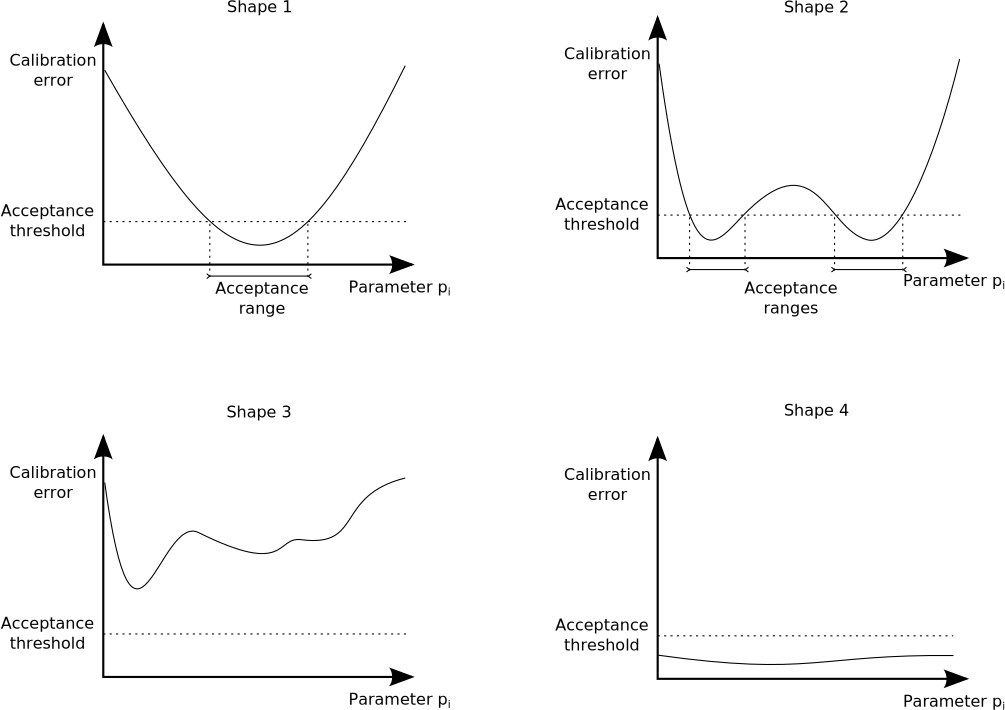
\includegraphics[width=\textwidth]{figures/profil_interpretation.png}
}


\sframe{Results}{

	\centering
	
	\includegraphics[width=\textwidth]{figures/PdiffusionZ.png}

}

\sframe{Results}{

	\centering
	
	\includegraphics[width=\textwidth]{figures/InnovationLife.png}

%Conclusion
%How to assess:

%the sufficiency of the mechanisms Y
%the necessity of the mechanisms Y
%the uniqueness of the mechanisms ?

}


\sframe{Unicity \cite{cottineau2014evolution}}{

%Automate the confrontation of alternative hypothesis / mechanisms.

\textit{Automate the confrontation of alternative hypothesis / mechanisms.}

\medskip

\centering
	
	\includegraphics[width=\textwidth]{figures/simfamily.png}

}


\sframe{Objective}{


%What we are running after?

\includegraphics[width=\textwidth]{figures/paretocomplexityfit.png}

}

\sframe{Multi-modeling (64 models)}{

%64 models

\centering

\includegraphics[width=0.8\textwidth]{figures/marius_complexification.png}

}


\sframe{Exemple of concurrent hypothesis}{


%Exchange mechanism:

%Market based
%Centrally planned

\textbf{Exchange mechanism: } market vs centralized

\medskip

%City growth mechanism:
%Purely inter-urban interactions
%Influenced by environmental situation

\textbf{City growth: } interurban interactions vs environmental situation

\medskip

\centering

\includegraphics[width=0.5\textwidth]{figures/system_mec.png}

}

\sframe{Calibration of model family}{

%
\textit{Compute the best set of parameters for all 64 models.}

\bigskip

\centering

\includegraphics[width=\textwidth]{figures/varius_big.png}

% http://shiny.parisgeo.cnrs.fr/VARIUS/

}



%
%\sframe{Calibration}{
%Calibration method
%Algorithm principle: reuse the good parameters found on one model to calibrate on the others.
%
%% Niched NSGA2 ?
%
%The method is tractable (even for ABMs):
%
%as fast (faster ??) as calibrating a single model.
%Handles stochasticity: 100x gain.
%Support for distributed computing: 1000x gain.
%
%%Conclusion
%%How to assess:
%
%%the sufficiency of the mechanisms Y
%%the necessity of the mechanisms Y
%%the uniqueness of the mechanisms (≈) Y
%
%Alternative approach
%All these methods are based on an a priori mesurement of the quality.
%
%Can we propose an alternative approach to evaluation?
%
%}




\sframe{Alternative approach: pattern search \cite{10.1371/journal.pone.0138212}}{

\centering

\includegraphics[width=\textwidth]{figures/pse_algo.png}

}

\sframe{Novelty search}{

%

\textit{The inputs producing rare patterns have high fitness values.}

\centering

\includegraphics[width=0.9\textwidth]{figures/hitmap.png}

}


\sframe{Results}{

\centering

\includegraphics[width=0.9\textwidth]{figures/flockingvolume.png}

}

\sframe{Results}{

\centering

\includegraphics[width=\textwidth]{figures/flockingpatterns.png}

}

\sframe{Results}{

\centering

\includegraphics[width=0.6\textwidth]{figures/pse_marius.png}

%Interpretation
%All expected/observed patterns are produced: the model is generic enough.
%
%
%Unexepected patterns are found:
%
%aberations: better constrain the model,
%predictions: test them.

% Exemple OpenMOLE + SimPLU (IGN) https://simplu.openmole.org/

}
%
%\sframe{Problème inverse}{
%\centering
%\includegraphics[width=\textwidth]{figures/ose_algo.png}
%}
%
%
%\sframe{Premiers résultats}{
%Formulation: $\Delta$ pattern < $\varepsilon$ %($f(x_1,\ldots, x_n) < 10$)
%\centering
%%\includegraphics[width=\textwidth]{figures/rastrigin.png}
%\includegraphics[width=\textwidth]{figures/oserast6d.png}
%%6-D Rastrigin function < 10
%}

% Want to use it?
%Stable: openmole.org
%Dev: next.openmole.org
%User forum: ask.openmole.org
%Source code: github.com/openmole/openmole
%Demo instance: demo.openmole.org
%Grid accesss: iscpif.fr/services



%Nous développons finalement les pistes de recherche qui en découlent et dans quelle mesures celles-ci s'intègrent au sein de perspectives plus larges de construction de disciplines intégrées et d'une interdisciplinarité accrue.


\section{Interactions between networks and territories}



\sframe{Interactions between networks and territories}{

\justify

\begin{center}

\includegraphics[width=\linewidth]{figures/example-tangjia.jpg}

\end{center}

\medskip

%\vspace{-0.5cm}

%\begin{justify}
\textit{Fieldwork observation of interactions between transportation and urban environment in Pearl River Delta: promotion of high speed, targeted urban development around stations.}

%\end{justify}

\nocite{raimbault2018evolving}

\medskip

\tiny

Raimbault, J. (2019). Evolving accessibility landscapes: mutations of transportation networks in China. In Aveline-Dubach, N., ed. \textit{Pathways of sustainable urban development across China - the cases of Hangzhou, Datong and Zhuhai}, pp 89-108. Imago. ISBN:978-88-94384-71-0

}




\sframe{Contrasted empirical observations}{

%Application de la méthode de caractérisation à des cas d'études à différentes échelles
%\bigskip

%\begin{columns}
%\begin{column}{0.5\textwidth}


	\includegraphics[width=\textwidth,height=0.8\textheight]{figures/empirical-southafrica.png}
	
	\smallskip
	
	
	\footnotesize
	
	%\vspace{-0.5cm}
	
	
	\begin{justify}
	\textit{Inversion of the sens of causality between population growth and railway accessibility increase in South Africa during the 20th century.}
	\end{justify}


%\end{column}
%\vrule\hspace{0.2cm}
%	\begin{column}{0.45\textwidth}

}



\sframe{Contrasted empirical observations}{


\begin{center}
	\includegraphics[width=0.8\textwidth]{figures/empirical-grdparis.jpg}
\end{center}	

	
	%\smallskip
	
	\footnotesize
	
	\vspace{-0.5cm}
	\begin{justify}
	\textit{Relations plus complexes dans le cas du gain d'accessibilité permis par le Grand Paris Express et les dynamiques socio-économiques des territoires}
	\end{justify}
	
	
%\end{column}
%\end{columns}

% LEGENDES

%\hspace{0.3cm}

}



\sframe{Modeling the co-evolution of networks and territories}{
	
	
	\textbf{Macroscopic scale:}
	\begin{itemize}
		\item Interaction models between cities including networks		
		$\rightarrow$ \textit{Demonstration of network effects; exploration\\
		 of interaction regimes}
	\end{itemize}

	\bigskip
	
	\uncover<2->{
	\textbf{Mesoscopic scale:}
	\begin{itemize}
		\item Urban morphogenesis model coupling urban form and network growth
		
		 $\rightarrow$ \textit{Complementarity of multiple processes; calibration at the first and second order}
		\item Exploration of a model including transportation governance
	\end{itemize}
}
	
}




\sframe{Mesoscopic models: morphogenesis}{


% - complementarité de multiples heuristiques de croissance de reseau
% - calibration au premier et second ordre
% - Lutecia : vers des modèles plus complexes


\footnotesize

%Relation entre forme et fonction (morphogenèse) comme paradigme pour modéliser la co-évolution à l'échelle mésoscopique.

%\smallskip

%\begin{columns}
%\begin{column}{0.55\textwidth}

%\footnotesize

\vspace{-0.8cm}

\justify
\textit{A morphogenesis model with reaction-diffusion and multi-modeling of network growth: complementarity of heuristics, calibration on forms and their correlations}

\medskip

{\centering
\includegraphics[width=0.25\linewidth,height=0.6\textheight]{figures/meso-nwgrowth.png}
\includegraphics[width=0.6\linewidth,height=0.6\textheight]{figures/meso-calib.jpg}
}

%\medskip

%$\rightarrow$ \textit{Complémentarité des heuristiques de réseau}
%  pour reproduire des formes existantes

%$\rightarrow$ \textit{Calibration sur les formes et leurs corrélations}

%\end{column}
%\vrule
%\hspace{0.2cm}
%\begin{column}{0.35\textwidth}

%\footnotesize

\bigskip

\tiny

Raimbault, J. (2018). Calibration of a density-based model of urban morphogenesis. PloS one, 13(9), e0203516.

\nocite{raimbault2018calibration}

\smallskip

Raimbault, J. (2019). An urban morphogenesis model capturing interactions between networks and territories. In The Mathematics of Urban Morphology (pp. 383-409). Birkhäuser, Cham.

\nocite{raimbault2019urban}

\smallskip

Raimbault, J. (2018). Multi-modeling the morphogenesis of transportation networks. In Artificial Life Conference Proceedings (pp. 382-383).


}




\sframe{A simple Reaction-diffusion model}{


\justify

$\rightarrow$ Crucial role of the interplay between concentration forces and dispersion forces~\cite{fujita1996economics} in keeping Urban Systems at the border of chaos

\bigskip

$\rightarrow$ Potentiality of aggregation mechanisms (such as Simon model) to produce power laws %\cite{2016arXiv160806313S}

\bigskip

$\rightarrow$ Link with Reaction-diffusion approaches in Morphogenesis~\cite{turing1952chemical}

\bigskip

$\rightarrow$ Extension of a DLA-type model introduced by \cite{batty1991generating}, with simple abstract processes of population aggregation and diffusion

}

\sframe{Model Formalization}{

% model formalization and indicators

$\rightarrow$ Grid world with cell populations $(P_i(t))_{1\leq i\leq N^2}$.

\bigskip

$\rightarrow$ At each time step:

% comment Arnaud : si tu beamais pas tu pourrais introduire une video du modèle ;-)

\begin{enumerate}
\item Population growth with exogenous rate $N_G$, attributed independently to a cell following a preferential attachment of strength $\alpha$
%\begin{equation}
%\Pb{P_i(t+1)=P_i(t)+1|P(t+1)=P(t)+1}=\frac{(P_i(t)/P(t))^{\alpha}}{\sum(P_i(t)/P(t))^{\alpha}}
%\end{equation}
%The attribution being uniformly drawn if all population are equal to 0.
\item Population is diffused $n_d$ times with strength $\beta$
\end{enumerate}

\bigskip

$\rightarrow$ Stopping criterion: fixed maximal population $P_m$.

%To avoid bord effects such as reflecting diffusion waves, border cells diffuse their due proportion outside of the world, implying that the total population at time $t$ is strictly smaller than $N_G\cdot t$.

\bigskip

$\rightarrow$ Output measured by morphological indicators: Moran index, average distance, rank-size hierarchy, entropy.


}


\sframe{Generating Population Distributions}{


% examples : fig 2 of paper

\centering

\includegraphics[height=0.8\textheight]{figures/density_Fig2}

\footnotesize\textit{Examples of generated territorial shapes}

}


\sframe{Model behavior}{

% comment Arnaud : Les graphiques correspondent aux 4 exemples précédents ? Si oui les rappeler en petite vignette. -> NON

\centering

\includegraphics[width=0.9\textwidth]{figures/density_Fig3}

\footnotesize\textit{Phase transitions of indicators unveiled by exploration of the parameter space (80000 parameter points, 10 repetitions each)}

% comment Arnaud : Préciser (dimensionner)

}




\sframe{Path-dependence and frozen accidents}{

\centering

\includegraphics[width=0.8\textwidth]{figures/density_Fig4}

\footnotesize\textit{Illustration of path-dependence in a simplified one-dimensional version of the model: cell trajectories in time for 9 independent repetitions from the same initial configuration.}


}


\sframe{Empirical Data for Calibration}{


\begin{columns}
\column{0.6\textwidth}
\centering
\includegraphics[width=\textwidth]{figures/density_indics_morpho_discrquantiles}
\column{0.3\textwidth}
\centering
\includegraphics[width=\textwidth]{figures/density_cluster_pca_k5_morpho}\\
\includegraphics[width=\textwidth]{figures/density_cluster_map_k5_morpho}
\end{columns}

\justify

\footnotesize\textit{Computation of morphological indicators on population density data for Europe (shown here on France), morphological classification.}

}



\sframe{Model Calibration}{

\includegraphics[width=\textwidth]{figures/density_synth}

\footnotesize\textit{Brute force calibration by exploring the parameter space. Reproduction of most existing configuration in the morphological sense (here in principal plan).}

}



\sframe{Model Targeted Exploration}{

\centering

\includegraphics[width=0.8\textwidth]{figures/density_Fig6}

\footnotesize\textit{Potentialities of targeted model explorations: here feasible space using Pattern Space Exploration algorithm \cite{10.1371/journal.pone.0138212}.}

}






\sframe{Including more complex processes ?}{

% transition : representation of territories

\textit{Which ontology to include more complex functional properties ?}

\medskip

$\rightarrow$ Territorial systems as the strong coupling between territories and (potential and realized) networks \cite{dupuy1987vers}.

\medskip

$\rightarrow$ Networks convey functional notions of centralities and accessibility, among others ; have furthermore proper topological properties.


}




\sframe{A Morphogenesis Model of co-evolution}{

\justify

\vspace{-1cm}

$\rightarrow$ Coupled grid population distribution and vector transportation network, following the core of \cite{raimbault2014hybrid}

\medskip

$\rightarrow$ Local morphological and functional variables determine a patch-value, driving new population attribution through preferential attachment ; combined to population diffusion (reaction-diffusion processes studied before)

% Comment Arnaud : réaction-diffusion ?

\medskip

$\rightarrow$ Network growth is also driven by morphological, functional and local network measures, following diverse heuristics corresponding to different processes (multi-modeling)

\bigskip
\bigskip

\textit{Local variables and network properties induce feedback on both, thus a strong coupling capturing the \textbf{co-evolution}}

}



\sframe{Model : Specification}{

\includegraphics[width=\textwidth]{figures/coevol_mesocoevol}

}



\sframe{Network Generation}{

At fixed time steps :

\begin{enumerate}
	\item Add new nodes preferentially to new population and connect them
	\item \justify Variable heuristic for new links, among: nothing, random, gravity-based deterministic breakdown, gravity-based random breakdown (from \cite{schmitt2014modelisation}), cost-benefits (from \cite{louf2013emergence}), biological network generation (based on \cite{tero2010rules})
\end{enumerate}

\medskip

\centering

\frame{\includegraphics[width=0.32\textwidth]{figures/example_nwgrowth_tick0.png}}
\frame{\includegraphics[width=0.32\textwidth]{figures/example_nwgrowth_tick2.png}}
\frame{\includegraphics[width=0.32\textwidth]{figures/example_nwgrowth_tick10.png}}

}




\sframe{Biological network generation}{

Model studied by~\cite{tero2010rules} : exploration and reinforcement by a slime mould searching for ressources

\bigskip

\includegraphics[width=0.32\textwidth]{figures/slimemould_tick1}
\includegraphics[width=0.32\textwidth]{figures/slimemould_tick10}
\includegraphics[width=0.32\textwidth]{figures/slimemould_tick20}\\
\includegraphics[width=0.32\textwidth]{figures/slimemould_tick50}
\includegraphics[width=0.32\textwidth]{figures/slimemould_tick101}
\includegraphics[width=0.32\textwidth]{figures/slimemould_reseauFinal}\\

\medskip

\footnotesize
\textit{Application to the design of optimal bus routes}

}




\sframe{Biological Network generation}{

Adding new links with biological heuristic:

\begin{enumerate}
	\item Create network of potential new links, with existing network and randomly sampled diagonal lattice
	\item Iterate for $k$ increasing ($k\in \{ 1,2,4 \}$ in practice) :
	\begin{itemize}
		\item Using population distribution, iterate $k\cdot n_b$ times the slime mould model to compute new link capacities
		\item Delete links with capacity under $\theta_d$
		\item Keep the largest connected component
	\end{itemize}
	\item Planarize and simplify final network
\end{enumerate}

\medskip

\centering

\frame{\includegraphics[width=0.6\textwidth]{figures/7-1-1-fig-networkgrowth-bioexample.jpg}}

\footnotesize

\textit{Intermediate stage for biological network generation}

}





\sframe{Generated Urban Shapes: Urban Form}{

\centering

\frame{\includegraphics[width=0.28\textwidth]{figures/coevol_example_synthsetup}}\hspace{0.1cm}
\frame{\includegraphics[width=0.28\textwidth]{figures/coevol_example_form-accessonly}}\hspace{0.1cm}
\frame{\includegraphics[width=0.28\textwidth]{figures/coevol_example_form-droadonly}}\\\vspace{0.1cm}
\frame{\includegraphics[width=0.28\textwidth]{figures/coevol_example_form-bwonly}}\hspace{0.1cm}
\frame{\includegraphics[width=0.28\textwidth]{figures/coevol_example_form-closenessonly}}\hspace{0.1cm}
\frame{\includegraphics[width=0.28\textwidth]{figures/coevol_example_form-poponly}}

\footnotesize\textit{In order: setup; accessibility driven; road distance driven; betweenness driven; closeness driven; population driven.}

}






\sframe{Generated Urban Shapes: Network}{


\centering

\frame{\includegraphics[width=0.28\textwidth]{figures/coevol_example_nw-connection}}\hspace{0.1cm}
\frame{\includegraphics[width=0.28\textwidth]{figures/coevol_example_nw-random}}\hspace{0.1cm}
\frame{\includegraphics[width=0.28\textwidth]{figures/coevol_example_nw-gravity}}\\\vspace{0.1cm}
\frame{\includegraphics[width=0.28\textwidth]{figures/coevol_example_nw-rndbrkdwn}}\hspace{0.1cm}
\frame{\includegraphics[width=0.28\textwidth]{figures/coevol_example_nw-cost}}\hspace{0.1cm}
\frame{\includegraphics[width=0.28\textwidth]{figures/coevol_example_nw-bio}}

\footnotesize\textit{In order: connection; random; deterministic breakdown; random breakdown; cost-driven; biological.}

}



\sframe{Results : Network Heuristics}{

\justify

\textit{Comparison of feasible space for network indicators with fixed density}

\bigskip

\includegraphics[width=0.52\textwidth,height=0.6\textheight]{figures/coevol_feasible_space_withreal_pca_bymorph}
\includegraphics[width=0.43\textwidth,height=0.6\textheight]{figures/coevol_distance_real_bymorph}

\footnotesize

\textit{(Left) Feasible spaces by morphological class and network heuristic; (Right) Distribution of distances to topologies of real networks}

}


\sframe{Results : Calibration}{

\justify

\vspace{-0.5cm}

Calibration (model explored with OpenMole~\cite{reuillon2013openmole}, $\sim 10^6$ model runs) at the first order on morphological and topological objectives, and on correlations matrices.

\bigskip

\begin{columns}
\column{0.4\textwidth}
\centering
\includegraphics[width=\textwidth]{figures/coevol_pca_allobjs}
\column{0.2\textwidth}
\includegraphics[width=\textwidth]{figures/coevol_pca_morpho_byheuristic}\\
\includegraphics[width=\textwidth]{figures/coevol_pca_network_byheuristic}
\column{0.4\textwidth}
\includegraphics[width=\textwidth]{figures/coevol_corrs-distrib_rhoasize4}

\end{columns}

\footnotesize\textit{(Left) Full indicator space; (Middle) Morphological and Topology, by network heuristic; (Right) Distance distribution for cumulated distance for indicators and correlations.}

}


\sframe{Results : Causality Regimes}{

\textit{Unsupervised learning on lagged correlations between local variables unveils a diversity of causality regimes}

$\rightarrow$ Link between \emph{co-evolution regime} and morphogenetic properties of the urban system

% comment Arnaud : le genre d’affirmation qu’il faut réussir à exprimer également du point de vue de l’objet étudié : qu’est-ce que ça veut dire pour la morphogénèse urbaine ?

\medskip

\centering

\includegraphics[width=0.52\textwidth,height=0.55\textheight]{figures/coevol_centertrajs}
\includegraphics[width=0.4\textwidth,height=0.55\textheight]{figures/coevol_cluster-params}

\footnotesize\textit{(Left) Lagged correlation profiles of cluster centers; (Right) Distribution of regimes across parameter space}

}





\sframe{Macroscopic interaction model}{

%\centering

\includegraphics[width=\textwidth]{figures/macrocoevol_model.png}


\nocite{raimbault2018indirect}
\nocite{raimbault2019modeling}

\vspace{-1cm}

\footnotesize

Raimbault, J. (2018). Indirect evidence of network effects in a system of cities. Environment and Planning B: Urban Analytics and City Science, 2399808318774335.

\smallskip

Raimbault, J. (2019). Modeling the co-evolution of cities and networks. In Niel, Z., Rozenblat, C., eds. \textit{Handbook of Cities and Network}, Edwar Elgar Publishing, \textit{in press}.


}






\sframe{Macroscopic Interaction Model Rationale}{

\justify

% bit of theory

\textbf{Rationale :} extend an interaction model for system of cities by including physical network as an additional carrier of spatial interactions 

\bigskip

$\rightarrow$ Work under Gibrat independence assumptions, i.e. $\Covb{P_i(t)}{P_j(t)}=0$. If $\vec{P}(t+1)=\mathbf{R}\cdot \vec{P}(t)$ where $\mathbf{R}$ is also independent, then $\Eb{\vec{P}(t+1)}=\Eb{\mathbf{R}}\cdot\Eb{\vec{P}}(t)$. Consider expectancies only (higher moments computable similarly)

\medskip

$\rightarrow$ With $\vec{\mu}(t)=\Eb{\vec{P}(t)}$, we generalize this approach by taking $\vec{\mu}(t+1)=f(\vec{\mu}(t))$


}


\sframe{Macroscopic Model Formulation}{

Let $\vec{\mu}(t)=\Eb{\vec{P}(t)}$ cities population and $(d_{ij})$ distance matrix


\medskip

Model specified by

\[
f(\vec{\mu}) = r_0\cdot \mathbf{Id}\cdot \vec{\mu} + \mathbf{G}\cdot \mathbf{1} + \mathbf{N}
\]

 with 
\begin{itemize}
\item $G_{ij} = w_G\cdot \frac{V_{ij}}{<V_{ij}>}$ and $V_{ij} = \left(\frac{\mu_i\mu_j}{\sum{\mu_k}^2}\right)^{\gamma_G} \exp{(-d_{ij}/d_G)}$
\item $N_{i} = w_N \cdot \sum_{kl} \left(\frac{\mu_k\mu_l}{\sum\mu}\right)^{\gamma_N}\exp{(-d_{kl,i})/d_N}$ where $d_{kl,i}$ is distance to shortest path between $k,l$ computed with slope impedance ($Z=\left(1+\alpha/\alpha_0\right)^{n_0}$ with $\alpha_0\simeq 3$)
\end{itemize}



}


\sframe{Data : stylized facts}{


Population data for French-cities (Pumain-INED database : 1831-1999)

% correlation curves, non-stationarity of network effects

\medskip

\textit{Non-stationarity of log-returns correlations function of distance}

\centering

\includegraphics[width=0.8\textwidth,height=0.7\textheight]{figures/intgib_Fig1}

}


\sframe{Geographic abstract network}{

% computation of geo shortest paths

\textit{Physical transportation network abstracted through a geographical shortest path network}

% map with shortest path examples

\medskip

\centering

\includegraphics[height=0.75\textheight]{figures/intgib_Fig2}

}

\sframe{Results : model exploration}{

% network effects graphs


\textit{Evidence of physical network effects : fit improve through feedback at fixed gravity}

\medskip

\centering

\includegraphics[width=\textwidth]{figures/intgib_Fig3}

}

\sframe{Results : model calibration}{

% ga calibration, both full model and gravity only

Model calibration using GA on computation grid, with software \texttt{OpenMole}~\cite{reuillon2013openmole}

\bigskip

\textit{Pareto front for full model calibration, objectives MSE and MSE on logs}

\medskip

\includegraphics[width=\textwidth,height=0.65\textheight]{figures/intgib_Fig4}

}

\sframe{Results : non-stationary gravity model calibration}{

% calibration on periods

\includegraphics[width=\textwidth,height=0.8\textheight]{figures/intgib_Fig5}

}


\sframe{Results : non-stationary full model calibration}{

% calibration on periods

\includegraphics[width=\textwidth,height=0.8\textheight]{figures/intgib_Fig6}

}

%
%\sframe{Quantifying overfitting : Empirical AIC}{
%
%\justify
%
%\vspace{-0.5cm}
%
%\textit{Not clear nor well theorized how to deal with overfitting in models of simulation.} \textbf{Intuitive idea : } Approximate gain of information by approaching models of simulation by statistical models.
%
%\medskip
%
%Let $M_k^{\ast} = M_k\left[\alpha_k^{\ast}\right]$ computational models heuristically fitted to the same dataset. With $S_k \simeq M_k^{\ast}$, we suppose that $\Delta D_{KL}\left( M_k^{\ast},M_{k'}^{\ast}\right) \simeq \Delta D_{KL}\left( S_k,S_{k'}\right)$ if fits of $S_k$ are negligible compared to fit difference between computational models and models have same parameter number.
%
%\bigskip
%
%\textbf{Application} $M_1$ : gravity only model with $(r_0=0.0133,w_G=1.28e-4,\gamma_G=3.82,d_G=4e12)$ ; $M_2$ : full model with $(r_0=0.0128,w_G=1.30e-4,\gamma_G=3.80,d_G=8.4e14,w_N=0.603,\gamma_N=1.148,d_N=7.474)$
%%Fitting of independent polynomial models ($\tilde{P}_i(t) = Q\left[\tilde{P}_i(t-1)\right]$) with 4 and 7 parameters) gives $\Delta D_{KL} \simeq 19.7$ $\rightarrow$ fit improvement without overfitting
%}


%\sframe{Empirical AIC values}{
%
%\begin{table}[ht]
%\caption{Empirical AIC results.}
%\begin{tabular}{|l|l|l|l|l|l}
%%\hrule
%Modèle Statistique &$M^{(1)}$ &$M^{(2)}$ & $\Delta AIC$ & $\Delta BIC$\\
%%\hrule
%Polynomial & 0.01438 & 0.01415 & 19.59 & 3.65\\
%Log-polynomial & 0.01565  & 0.01435 & 125.37 & 109.43\\
%Polynomial Généralisé & 0.01415  & 0.01399 & 11.70 & -4.23\\
%%\hrule
%\end{tabular}
%\end{table}
%}



%%%%%%%%%%%%%%
% \section*{Macro co-evolution}



\sframe{Generic Model}{

% idea : present it with a schema : YES.

\centering

\includegraphics[width=\textwidth]{figures/macrocoevol_model.pdf}

}





\sframe{Model Formalization : Network Growth}{

Given the flow $\phi$ in a link, its effective distance is updated following

\begin{enumerate}
\item For the thresholded case
\[
d(t+1) = d(t)\cdot \left( 1 + g_{max} \cdot \left[\frac{1 - \left(\frac{\phi}{\phi_0}\right)^{\gamma_s}}{1 + \left(\frac{\phi}{\phi_0}\right)^{\gamma_s}}\right]\right)
\]
\item For the full growth case
\[
d(t+1) = d(t)\cdot \left(1 + g_{max} \cdot \left[\frac{\phi}{\max \phi}\right]^{\gamma_s}\right)
\]
\end{enumerate}

where $\gamma_s$ is a hierarchy parameter, $\phi_0$ a threshold parameter and $g_{max}$ the maximal growth rate easily adjustable to realistic values by computing $(1+g_{max})^{t_f}$



}


\sframe{Model Formalization : Indicators}{
  \begin{itemize}
  \item Hierarchy, Entropy, Summary statistics in time
  \item Initial-final rank correlation (changes in the hierarchy) for variable $X$ : $\rho\left[X_i(t=0),X_i(t=t_f)\right]$
  \item Trajectory diversity for variable $X$ : with $\tilde{X}_i(t)\in \left[0;1\right]$ rescaled trajectories,
  \[
    \frac{2}{N\cdot(N-1)}\sum_{i<j} \left(\frac{1}{T}\int_{t} \left(\tilde{X}_i(t) - \tilde{X}_j(t)\right)^2 \right)^{\frac{1}{2}}
  \]
  \item Average trajectory complexity (number of inflexion points)
  \item Pearson correlations conditionally to distance $\hat{\rho}_d\left[(X(\vec{x}_1,Y(\vec{x}_2))|||\vec{x}_1-\vec{x}_2||\sim d\right]$
  \item Lagged return correlations $\hat{\rho}_{\tau}\left[\Delta X(t),\Delta Y(t-\tau)\right]$ (Granger causality)
  \end{itemize}
}


\sframe{Model Specification : Abstract Network}{
 % description + illustration (t0, tf)
 
 \textit{Complete virtual network between cities, initialized with euclidian distances ; thresholded reinforcement of speeds as a function of flows.}
 
 \bigskip
 
 \centering
 
 \includegraphics[width=0.4\textwidth]{figures/macrocoevol_example_virtual_0_t0}\hspace{0.2cm}
 \includegraphics[width=0.4\textwidth]{figures/macrocoevol_example_virtual_0_tf}
 
 {\small\textit{Exemple of run ($t_f=30$). Level of red gives overall growth and link width flows.}}
 
}

\sframe{Results: emergence of co-evolution niches}{

\begin{center}
\includegraphics[width=0.75\linewidth,height=0.75\textheight]{figures/macrocoevol_Fig3.jpg}
\end{center}


\medskip

\textit{Trajectories of maximal complexity for intermediate values of interaction range.}

}




\sframe{Results: co-evolution regimes}{

%\begin{column}{0.3\textwidth}

\begin{center}

	\includegraphics[width=\linewidth]{figures/macro-regimes.png}
	
	\medskip
	
	%\footnotesize
	
	%\begin{justify}

\end{center}


\vspace{-0.4cm}

	\textit{Multiple co-evolution regimes highlighted for synthetic urban systems, using the PSE diversity search algorithm}


	%\end{justify}
%\end{column}


}







\sframe{Other example of multi-modeling}{

\textit{Benchmark of growth models for systems of cities} \cite{raimbault2018systematic}

\centering

\includegraphics[width=0.9\textwidth]{figures/CN_zoomed.png}

}










%
%
%
%
%
\sframe{Conclusion}{

$\rightarrow$ Multiple ways to model urban systems and to extract knowledge from these: \textbf{towards more coupling and comparison of models.}

\smallskip

$\rightarrow$ At which scale ? \textbf{Need for multi-scale models.}

\smallskip

$\rightarrow$ With more refined urban characteristics and other dimensions? \textbf{Need for more interdisciplinarity.}


\bigskip
\bigskip

\textbf{To use OpenMOLE (free and open software) and contribute: }
\url{next.openmole.org}

\bigskip
\bigskip

%
%
%\justify
%
%%\vspace{-1cm}
%
%%$\rightarrow$ 
%
%\textit{Significant accomplishments beyond disciplines, construction of new research practices (see the satellite presentations)} $\rightarrow$ still much to do ? (e.g. how to put into practice ? how to achieve true integration ? etc.)
%

%\textit{Accomplissements significatifs au-delà des disciplines, construction de nouvelles pratiques de validation des modèles}

%\medskip

% $\rightarrow$ encore beaucoup à faire : comment atteindre un réelle intégration ? comment faire percoler les pratiques dans d'autres disciplines ? Quel changement institutionnel ? Epistémologique ? \cite{pumain2018from}

%\bigskip
%
%\textbf{\textit{``La route est longue mais la voie est libre''}}
%
%\bigskip
%
%\textbf{\textit{You need OpenMOLE and OpenMOLE needs you !}} (win-win interdisciplinary relations):
%\textbf{École d'été OpenMOLE} \texttt{https://exmodelo.org/}
%
%\bigskip
%\bigskip
%\bigskip

%\footnotesize
%
\textbf{Some references}

\medskip

\tiny

%Raimbault, J. (2017, December). An Applied Knowledge Framework to Study Complex Systems. In Complex Systems Design \& Management (pp. 31-45). arXiv:1706.09244.
%
%\medskip


Raimbault, J. (2018). Caract{\'e}risation et mod{\'e}lisation de la co-{\'e}volution des r{\'e}seaux de transport et des territoires (Doctoral dissertation, Université Paris 7 Denis Diderot). \url{https://halshs.archives-ouvertes.fr/tel-01857741}

\smallskip

Raimbault, J. (2018). Indirect evidence of network effects in a system of cities. Environment and Planning B: Urban Analytics and City Science, 2399808318774335.

\smallskip

Raimbault, J. (2018). Calibration of a density-based model of urban morphogenesis. PloS one, 13(9), e0203516.

\smallskip

Raimbault, J. (2019). An urban morphogenesis model capturing interactions between networks and territories. In The Mathematics of Urban Morphology (pp. 383-409). Birkhäuser, Cham.



%
%
%
%
%%\smallskip
%
%%\textbf{Open repository} at \texttt{https://github.com/JusteRaimbault/UrbanGrowth}\\\smallskip
%%\textbf{Acknowledgments}: thanks to the \textit{EGI} for access to the infrastructure.
%
%
}
%
%



\sframe{OpenMOLE summer school}{

\includegraphics[width=\linewidth]{figures/exmodelobanner.png}

\medskip

\textit{Next week is our summer school, soon receiving applications for next year}

\url{exmodelo.org}

}


\sframe{Submit to special session at CCS}{


\includegraphics[width=\linewidth]{figures/ccs.png}

\medskip

\textit{Satellite session on methods and epistemology in modeling and simulation, at Conference on Complex Systems, 2nd October 2019}

\smallskip

\textbf{Submit your abstract before June 30th !}

\url{https://iscpif.fr/ccs-satelllite-session-2019-new-methods/}

\smallskip

\textbf{Submission link:}

\url{https://easychair.org/conferences/?conf=simexplo2019}

}







\sframe{Reserve slides}{

\centering

\Large

\textbf{Reserve Slides}

}



%%%%%%%%%%%%%%%%%%%%%
\begin{frame}[allowframebreaks]
\frametitle{References}
\bibliographystyle{apalike}
\bibliography{/Users/juste/ComplexSystems/CityNetwork/Biblio/Bibtex/CityNetwork,biblio}
\end{frame}
%%%%%%%%%%%%%%%%%%%%%%%%%%%%






\sframe{Model classification : PDE}{

% derived PDE

The one-dimensional model verifies the PDE :

\begin{equation}\label{eq:pde}
\begin{split}
\delta t \cdot \frac{\partial p}{\partial t} = \frac{N_G \cdot p^{\alpha}}{P_{\alpha}(t)} + \frac{\alpha \beta (\alpha - 1) \delta x^2}{2}\cdot \frac{N_G \cdot p^{\alpha-2}}{P_{\alpha}(t)} \cdot \left(\frac{\partial p}{\partial x}\right)^2\\
+ \frac{\beta \delta x^2}{2} \cdot \frac{\partial^2 p}{\partial x^2} \cdot\left[ 1 + \alpha \frac{N_G p^{\alpha - 1}}{P_{\alpha(t)}} \right]
\end{split}
\end{equation}

}


\sframe{Stationary behavior of 1D model}{
\centering
\includegraphics[width=\textwidth]{figures/density_stationary}
}

\sframe{Stationary behavior of 1D model}{
\centering
\includegraphics[width=0.48\textwidth]{figures/density_pmax_alpha}
\includegraphics[width=0.48\textwidth]{figures/density_pmax_logbeta}

}



\sframe{Morphological indicators}{

\begin{enumerate}
\item Rank-size slope $\gamma$, given by $\ln \left( P_{\tilde{i}}/P_0\right) \sim k + \gamma\cdot \ln \left(\tilde{i}/i_0\right)$ where $\tilde{i}$ are the indexes of the distribution sorted in decreasing order.
\item Entropy of the distribution:
\begin{equation}
\mathcal{E} = \sum_{i=1}^{M}\frac{P_i}{P}\cdot \ln{\frac{P_i}{P}}
\end{equation}
$\mathcal{E}=0$ means that all the population is in one cell whereas $\mathcal{E}=0$ means that the population is uniformly distributed.
\item Spatial-autocorrelation given by Moran index, with simple spatial weights given by $w_{ij} = 1/d_{ij}$
\[
I = M \cdot \frac{\sum_{i\neq j} w_{ij} \left(P_i - \bar{P}\right)\cdot\left(P_j - \bar{P}\right)}{\sum_{i\neq j} w_{ij} \sum_{i}{\left( P_i - \bar{P}\right)}^2}
\]
\item Mean distance between individuals
\[
\bar{d} = \frac{1}{d_M}\cdot \sum_{i<j} \frac{P_i P_j}{P^2} \cdot d_{ij}
\]
where $d_M$ is a normalisation constant
\end{enumerate}



}


\sframe{Model behavior : Convergence}{

Large number of repetitions show good convergence properties

% hist examples

\includegraphics[width=0.5\textwidth]{figures/density_hist_moran}
\includegraphics[width=0.5\textwidth]{figures/density_hist_slope}

}


\sframe{Model behavior}{


\includegraphics[width=0.5\textwidth]{figures/density_pc_colalpha}
\includegraphics[width=0.5\textwidth]{figures/density_pc_colbeta}

}


\sframe{Empirical indicators computation}{

$\rightarrow$ Eurostat population density raster (100m, simplified at 500m resolution)

\medskip

$\rightarrow$ Overlapping (10km offset) squares of 50km side : equivalent to smoothing, removes window shape effect. Not very sensitive to window size (tested with 30km and 100km)

\medskip

$\rightarrow$ Indicators computed using Fast Fourier Transform Convolution

\medskip

$\rightarrow$ Classification using repeated k-means ; number of clusters taken at transition in clustering coefficient.

}

\sframe{Model calibration: all indicators}{

\centering
\includegraphics[width=0.8\textwidth]{figures/density_scatter}

}







\sframe{Model parameters}{

\centering

\vspace{-0.2cm}
\begin{tabular}{|p{1.5cm}|c|c|c|c|c|}
  \hline
Heuristic & Param. & Name & Process & Domain & Default\\
  \hline
\multirow{5}{*}{Base}& $l_m$ & added links & growth & $[0;100]$ & $10$ \\\cline{2-6}
 & $d_G$ & gravity distance & potential & $]0;5000]$ & $500$ \\\cline{2-6}
 & $d_0$ & gravity shape & potential & $]0;10]$ & $2$ \\\cline{2-6}
 & $k_h$ & gravity weight & potential & $[0;1]$ & $0.5$ \\\cline{2-6}
 & $\gamma_G$ & gravity hierarchy & potential & $[0.1;4]$ & $1.5$ \\\hline
\multirow{2}{*}{Random}& $\gamma_R$ & random selection  & hierarchy & $[0.1;4]$ & $1.5$ \\\cline{2-6}
& $\theta_R$ & random threshold & breakdown & $[1;5]$ & $2$ \\\hline
Cost-benefits & $\lambda$ & compromise & compromise & $[0;0.1]$ & $0.05$ \\\hline
\multirow{2}{*}{Biological}& $n_b$ & iterations & convergence & $[40;100]$ & $50$ \\\cline{2-6}
& $\theta_b$ & biological th.& threshold & $[0.1;1.0]$ & $0.5$ \\\hline
\end{tabular}

}



\sframe{Model setup}{

\textbf{Synthetic setup: } rank-sized monocentric cities, simple connection with bord nodes to avoid bord effects 

\textbf{Real setup: } Population density raster at 500m resolution (European Union, from Eurostat)

\bigskip

\centering
\frame{\includegraphics[width=0.35\textwidth]{figures/coevol_example_synthsetup}}\hspace{0.1cm}
\frame{\includegraphics[width=0.35\textwidth]{figures/coevol_example-realsetup}}

\textbf{Stopping conditions: } fixed final time; fixed total population; fixed network size.

}


\sframe{Network Indicators}{

Network Topology measured by:

\begin{itemize}
	\item Betweenness and Closeness centralities: average and hierarchy
	\item Accessibility (weighted closeness)
	\item Efficiency (network pace relative to euclidian distance)
	\item Mean path length, diameter
\end{itemize}

}



\sframe{Network nodes}{

\textbf{Network baseline extension:}

Adding a fixed number $n_N$ of new nodes : for patches such that $d_r < d_0$, probability to receive a node is

% note : not a proba for the last ? no pb as soon as in 0,1, realized anyway.
\[
p = P/P_{max} \cdot (\delta_M - \delta)/\delta_M
\]
% \cdot \exp\left(-((d_r - d_0)/\sigma_r)^2\right)


Nodes connected the shortest way to existing network.

}



\sframe{Biological network morphogenesis model}{

Model studied by~\cite{tero2010rules}: exploration and reinforcement by a slime mould searching for ressources

\medskip

Settings :
\begin{itemize}
	\item Initial homogeneous network of tubes $ij$ of length $L_{ij}$, variable diameter $D_{ij}$, carrying a flow $Q_{ij}$.
	\item Nodes $i$ with a pressure $p_i$.
	\item $N$ nodes are origin/destination points : randomly at each step one becomes source $p_{i_+}=I_0$ and one other sink $p_{i_-}=-I_0$
\end{itemize}


}

\sframe{Biological network evolution}{

At each iteration :
\begin{enumerate}
	\item Determination of flows with Kirchoff's law (electrostatic analogy) : Ohm's law $Q_{ij}=\frac{D_{ij}}{L_{ij}}\cdot(p_{i}-p_{j})$ and conservation of flows $\sum_{j\rightarrow i}Q_{ij} = 0 , \sum_{j\rightarrow i_\pm}Q_{i_{\pm}j} = \pm I_0$
	\item Evolution of diameters ($\gamma$ reinforcement parameter) by
	\[
	\frac{dD_{ij}}{dt}=\frac{\left|Q_{ij}\right|^{\gamma}}{1+\left|Q_{ij}\right|^{\gamma}}-D_{ij}
	\]
\end{enumerate}

\medskip


$\rightarrow$ Extraction of the final network after convergence given a threshold parameter for diameters %(bimodal final distributions)

\medskip

$\rightarrow$ Multi-scale model : diameters are constant during an iteration to obtain equilibrium flows

}



\sframe{Biological network: indicators}{

Behavior of the model evaluated with performance indicators for generated network $(V_f,E_f)$, that are contradictory objectives :
          \bigskip
          \begin{itemize}
          \item Construction costs $c=\sum_{ij\in E_f}D_{ij}(t_f)$
          \bigskip
          \item \begin{justify}Average performance~\cite{banos2012towards}
          \[
          v=\frac{1}{|V_f|^2}\sum_{i,j\in V_f}\frac{d_{i\rightarrow j}}{||\vec{i}-\vec{j}||}
          \]
          \end{justify}
          \bigskip
          \item Robustness (\textit{Network Trip Robustness} index~\cite{sullivan2010identifying})
          \end{itemize}

}


\sframe{Biological network: optimal networks}{

\centering

%\includegraphics[height=0.8\textheight]{figures/slimemould_paretoSpeedLength.png}
\includegraphics[height=0.8\textheight]{figures/pareto_cost-robustness_facetCenterNumber_withgaussianCI.png}


\footnotesize \textit{Exploration of parameter space for synthetic network generation}

}





\sframe{Deterministic breakdown Network generation}{

\begin{enumerate}
\item Gravity potential given by
\[
V_{ij}(d) = \left[ (1 - k_h) + k_h \cdot \left( \frac{P_i P_j}{P^2} \right)^{\gamma} \right]\cdot \exp{\left( -\frac{d}{r_g (1 + d/d_0)} \right)}
\]

\item $k\cdot N_L$ links are selected with lowest $V_{ij}(d_N)/V_{ij}(d_{ij})$, among which $N_L$ links with highest (lest costly) are realized
\item Network is planarized
\end{enumerate}
}





\sframe{Results: components}{

With average betweenness centrality $\bar{bw}$ and average closeness centrality $\bar{cl}$, diameter $r$, average path length $\bar{l}$, relative speed $v_0$

\medskip

\textbf{Simulated point cloud:} $PC1 = - 0.51 \bar{bw} - 0.45 \bar{l} + 0.57 v_0 - 0.43 r + 0.05 \bar{cl}$ and $PC2 = -0.45 \bar{bw} + 0.17 \bar{l} +0.33 v_0 + 0.8 r +0.1 \bar{cl}$

\medskip

\textbf{Herfindhal index} (20 width grid): first quartile at $0.54$, a median at $0.76$ and a third quartile at $1$

\medskip

\textbf{Distance to real configurations:} $d(1,2) = \sqrt{(\bar{bw}_1 - \bar{bw}_2)^2 + (\bar{cl}_1 - \bar{cl}_2)^2 + (\bar{l}_1 - \bar{l}_2)^2}$, we use $d_{min} = \min_j d(S,R_j)$

\medskip

\textbf{Real point cloud:} $PC1 = 0.12 \bar{bw} - 0.09 \bar{cl} + 0.98 \bar{l}$ and $PC2 = -0.20 \bar{bw} - 0.97 \bar{cl} - 0.06 \bar{l}$


}

\sframe{Population morphology classes}{

With 10 grids per class:
\begin{itemize}
	\item Class 5: lowest Moran, high distance, hierarchy and entropy; numerous population centers that are localized and dispersed.
	\item Class 4: highest entropy and hierarchy; a small number of localized centers.
	\item Class 3: lowest distance and entropy; diffuse population.
	\item Class 2: highest Moran; one or a few centers with consequent size.
	\item Class 1: intermediate values for all indicators; a certain number of centers of intermediate size.
\end{itemize}

}


\sframe{Population morphology classes}{

\centering

\begin{tabular}{|c|c|c|c|c|}
\hline
Class & Moran $I$ & Distance $\bar{d}$ & Entropy $\mathcal{E}$ & Hierarchy $\gamma$ \\\hline 
1 & 0.23 & 0.66 & 0.76 & 0.62 \\\hline % medium everything
2 & 0.47 & 0.50 & 0.75 & 0.53 \\\hline % highest moran, medium others
3 & 0.21 & 0.42 & 0.57 & 0.65 \\\hline % lowest distance and entropy, medium slope
4 & 0.24 & 0.75 & 0.90 & 0.87 \\\hline % highest entropy and slope
5 & 0.15 & 0.76 & 0.84 & 0.72 \\\hline % lowest moran, high distance, slope and entropy
\end{tabular}

}












\end{document}













\sframe{Résumé du positionnement d'OpenMOLE}{

%\textit{A qualitative shift in knowledge that can be extracted from a simulation model with model exploration methods.}

\textit{Un saut qualitatif dans la connaissance extraite d'un modèle de simulation par les méthodes d'exploration des modèles}

\medskip

%Success stories: SimpopLocal \cite{schmitt2014half}, Marius \cite{10.1371/journal.pone.0138212}, Ecological modeling \cite{lavallee2018dynamical}, epidemiology \cite{arduin2018modelisation}, etc.

Réussites: SimpopLocal \cite{schmitt2014half}, Marius \cite{10.1371/journal.pone.0138212}, modélisation en écologie \cite{lavallee2018dynamical}, en épidémiologie \cite{arduin2018modelisation}, etc.

\medskip

\textbf{Caractéristiques principales: }

\begin{itemize}
	%\item Unique role of complementary axis of computation environment access, methods providing, and model embedding.
	\item Role unique des axes complémentaires de l'accès aux environnements, de la disponibilité des méthodes, et de l'embarquement des modèles.
	%\item Iterative and integrated construction of models and theories, using all dimensions of knowledge enhanced by simulation and computation (modeling, theory, empirical, data, methods, tools \cite{raimbault2017applied}.
	\item Construction itérative et intégrée des modèles et théories, en utilisant l'ensemble des dimensions de la connaissance favorisées par la simulation et le calcul (modélisation, théorie, empirique, données, méthodes, outils \cite{raimbault2017applied}).
	%\item Coupling models and reproducibility at the core of the workflow approach \cite{passerat2017reproducible}
	\item Couplage des modèles et reproductibilité au coeur de l'approche par workflow \cite{passerat2017reproducible}.
\end{itemize}


}


%
\sframe{Tendances et défis actuels en (géo-)simulation}{

%% 
%%\centering
%%\justify
%
%% We first survey the current trends and explicit the positioning of OpenMOLE's philosophy within these.
%
%\textbf{Key domains: } quantifying urban growth and form, mining spatio-temporal data, geosimulation, multi-scalar approaches \cite{behnisch2018trends}.
\textbf{Domaines principaux: } quantification de la croissance et de la forme urbaine, fouille de données spatio-temporelles, géosimulation, approches multi-scalaires \cite{behnisch2018trends}.


\medskip

\textbf{Défis: }
%
\begin{itemize}
%	\item \cite{perez2016agent} key challenges in ABM for planning: addressing complexity in a clean way, addressing multi-dimensionality, feasible trajectories, participatory planning.
	\item Cas des ABM pour la planification \cite{perez2016agent} : complexité simplifiée, multi-dimensionnalité, trajectoires faisables, planification participative
%	\item Simulation models \cite{banos2013pour}: interdiscplinarity, data-driven models, exploration of models, multi-objective issues, reproducibility and reuse of models, coupling models.
	\item Modèles de simulation \cite{banos2013pour}: interdisciplinarité, modèles ancrés dans les données, exploration des modèles, problèmes multi-objectifs, reproductibilité et réutilisation des modèles, couplage des modèles.
\end{itemize}
%
%
\medskip
%
%\textbf{Future ?} \cite{banos2017knowledge} deeper and integrated knowledge; \cite{arribas2018geography} new geographic data science?

\textbf{Futur ?} \cite{banos2017knowledge} connaissance plus profonde et intégrée; \cite{arribas2018geography} vers une nouvelle science géographique des données ?

}




\sframe{Questions ouvertes pour la simulation en TQG}{

%
%%We then propose a grasp on some future perspectives, by detailing examples of crucial research questions on simulation models in geography that remain open, including in particular, first generic issues such as
%
%% plan (generic + specific to spatio-temporal modeling)
%
%\textit{Some of crucial issues :}
%
%\medskip
%
\textbf{Question générales: }
\begin{itemize}
	\item Surajustement des modèles de simulation
	\item Couplage des modèles
	\item Comportement direct et indirect
	\item Stochasticité
\end{itemize}

\medskip

\textbf{Spécifiques aux systèmes spatio-temporels: }
\begin{itemize}
	\item Non-stationnarité spatio-temporelle
	\item Données synthétiques spatio-temporelles
\end{itemize}




}


%
%
%
\sframe{Surajustement}{
%
%% (i) the development of multi-modeling techniques that explicitly account for overfitting for simulation models;
%\textit{When do additional parameters actually capture new dimensions of the simulated system ? i.e. when does fit improvement is not only due to more degree of freedom ?}
\textit{Dans quel mesure l'ajout de paramètres améliore effectivement l'information extraite ?}

%
\medskip
%
%$\rightarrow$ Crucial for parcimonious models, which can be used then as building bricks for more complex models.
%
$\rightarrow$ Fondamental pour des modèles parcimonieux, qui peuvent ensuite être utilisés comme briques pour des modèles plus complexes.

\medskip
%
\begin{itemize}
%	\item Black-box brutal data explanation ?
	\item Pouvoir explicatif brutal ``boîte-noire'' ?
%	\item Extension of AIC-type measures ?
	\item Extension de mesures de type AIC ?
%	\item Multi-objective optimisation with degrees of freedom ?
	\item Optimisation multi-objectif incluant degrés de liberté ?
\end{itemize}
%
% RQ : encore le lien aggreg / multidim optim ici !
%
}

%
\sframe{Couplage de modèles}{
%
%% (ii) a better understanding of model coupling
%% (includes multi-scale more or less)
%% -> robust definition / classification of models etc
%
%\textit{Definition/theory/quantification of model coupling ?}
%
\textit{Définition/théorie/quantification du couplage de modèles ?}

\medskip
%
%$\rightarrow$ Crucial for interdisciplinarity, reproducibility and the reuse of models; crucial for multi-scalar approaches (downward causation); crucial for model benchmarking.

$\rightarrow$ Fondamental pour l'interdisciplinarité, la reproductibilité et la réutilisation des modèles; pour les approches multi-scalaires (rôle de la causalité descendante); pour le comparaison de modèles.

\medskip

\begin{itemize}
%	\item Model-independent notion of ``coupling-strength'' ?
	\item Notion de ``force de couplage'' indépendante des modèles ?
%	\item Covariance structures ?
	\item Structures de covariance ?
%	\item Causal graphs ?
	\item Graphes causaux ?
\end{itemize}

}


\sframe{Comportement direct et indirect}{
%
%% (iii) the development of adaptative direct and inverse mapping methods;
%% inverse problems / feasible space
%
%\textit{How to have a comprehensive overview of strongly non-linear simulation models mapping ?}
%
\textit{Comment obtenir un aperçu relativement exhaustif du comportement d'un modèle de simulation fortement non-linéaire ?}

\medskip

%$\rightarrow$ Feasible space and unexpected patterns (PSE algorithm \cite{10.1371/journal.pone.0138212}); dealing with equifinality.

$\rightarrow$ Espace faisable et motifs inattendus (algorithme PSE \cite{10.1371/journal.pone.0138212}); question de l'équifinalité.

\medskip

\begin{itemize}
	%\item Inverse problem heuristics being currently tested in OpenMOLE
	\item Heuristiques de problème inverse en cours d'expérimentation
	%\item Iterative approach to determine main patterns in the mapping ?
	\item Approche itérative pour extraire les motifs principaux de comportement
\end{itemize}

}


\sframe{Gestion de la stochasticité}{

%% (iv) a better handling of stochasticity in ``real-world'' models;
%
%\textit{How to handle stochastic models during genetic algorithm calibration or exploration ?}

\textit{Quelle place et quelle gestion de la stochasticité dans la construction et l'exploration des modèles ?}

% rq : un peu plus general que juste GA ; lie à structure covariance - matrice interaction

\medskip
%
%$\rightarrow$ Crucial for more data-driven and ``real-world'' models; crucial for a robust knowledge extracted from simulation models.
%

$\rightarrow$ Fondamental pour des modèles basé sur les donnés et appliqués; pour une connaissance robuste extraite des modèles de simulation.

\medskip
%
\begin{itemize}
%	\item Deal with ``real-world'' noise patterns
	\item Prise en compte de bruits ``réels''
%	\item An embedding approach tested in OpenMOLE to deal with noisy fitness
	\item Une approche par augmentation de la dimension en cours de test
%	\item A bayesian approach to calibration (ABC) also currently tested
	\item De même, une approche bayesienne de la calibration (ABC)
\end{itemize}


}

\sframe{Modélisation spatio-temporelle: non-stationnarité}{
%
%%  and secondly issues which are more specific to spatio-temporal models, such as (v) the understanding of spatio-temporal non-stationarity, possibly through the intermediate of limit links between agent-based approaches and system dynamics approaches;
%
%\textit{How to understand and include spatio-temporal non stationarity in empirical analysis / in model simulations and calibration ?}

\textit{Comment inclure la non-stationnarité spatio-temporelle dans les analyses empiriques, les simulations et calibrations de modèles ?}


\medskip

%$\rightarrow$ Intrinsic complexity of spatial systems; crucial for multi-scalar approaches.
%
$\rightarrow$ Complexité intrinsèque des systèmes spatiaux; fondamental pour les approches multi-scalaires.

\medskip

\begin{itemize}
%	\item Link between non-stationarity and non-ergodicity
	\item Lien entre non-stationnarité et non-ergodicité
%	\item Link between ABM approaches and dynamical systems approaches, towards hybrid approaches \cite{banos2015importance}
	\item Lien entre approches basées sur les agent et systèmes dynamiques, vers des approches hybrides \cite{banos2015importance}
\end{itemize}


}

%
\sframe{Données synthétiques spatio-temporelles}{

%% and (vi) methods to generate synthetic spatio-temporal data to be used for broader sensitivity analyses.

%\textit{How to extend sensitivity analyses to spatial initial conditions ? How to generate spatial synthetic data ?}

\textit{Comment étendre les analyses de sensibilité aux conditions spatiales initiales ? Comment générer des données spatiales synthétiques ?}


\medskip

%$\rightarrow$ Crucial for the robustness of spatial simulations

$\rightarrow$ Fondamental pour la robustesse des simulations spatiales

\medskip

\begin{itemize}
%	\item First work in the case of density grids in territorial systems \cite{cottineau2017initial}
	\item Première approche dans le cas de grilles de densité de population \cite{cottineau2017initial}
%	\item Extend to other disciplines: ecology, geosciences
	\item Extension à d'autres disciplines: écologie, géosciences
%	\item Towards a generic library integrated in OpenMOLE
	\item Vers une bibliothèque générique intégrée à OpenMOLE
\end{itemize}

}


%
%
%
%\sframe{An integrated view}{
%	
%	% graph between different open issues
%	
%	\includegraphics[width=\textwidth]{figures/directions.pdf}
%	
%}
%
%


\sframe{Cadre: domaines de connaissance}{

%Applied knowledge framework proposed by \cite{raimbault2017applied} to study [complex] systems

Cadre de connaissance appliqué \cite{raimbault2017applied} %pour l'étude des systèmes [complexes]

\medskip

\centering

\includegraphics[width=0.8\textwidth]{figures/framework_fr.pdf}

}



\sframe{Un perspectivisme appliqué pour coupler les approches}{
%
%% We finally describe an epistemological framework integrating several of these issues, which applies Giere's perspectivism to the effective coupling of simulation models, and that we call ``applied perspectivism''. This framework should foster the development of integrative theories through the coupling of perspectives, and therefore of models.
%
%% link it with knowledge framework
%
%Perspectivisme de Giere \cite{giere2010scientific}: a ``third way'' beyond constructivism-realism: \textit{Any scientific knowledge construction process as a perspective by an agent to answer a purpose with a media (model)}.
\textbf{Perspectivisme de Giere} \cite{giere2010scientific}: une ``troisième voie'' au delà de la dichotomie constructivisme-réalisme. \textit{Tout processus de construction d'une connaissance scientifique comme une perspective par un agent pour répondre à un but par l'intermédiaire d'un medium (le modèle)}. [Compatible avec l'approche fonctionnelle de \cite{varenne2017theories}]

% rq : coupplage Giere-Varenne base d'une approche de modelisation - socio-evidence based ?


\medskip

%Applied knowledge framework proposed by \cite{raimbault2017applied} to study [complex] systems: \textit{co-evolution} of cognitive agents and knowledge domains, through the intermediate of perspectives.

\textbf{Agents cognitifs et les domaines de connaissance sont en \textit{co-évolution}, par l'intermédiaire des domaines de connaissance.}

\medskip

\textbf{Principes du perspectivisme appliqué:}
\begin{itemize}
	%\item Foster consistence of perspectives and their communication (Banos' virtuous spiral between disciplinarity and interdisciplinarity)
	\item Favoriser la cohérence des perspectives et leur communication (spirale vertueuse de Banos entre disciplinarité et interdisciplinarité)
	%\item Importance of reflexivity to ease the coupling of perspectives
	\item Importance de la réflexivité pour faciliter le couplage des perspectives
	%\item New model exploration methods increase the integration between knowledge domains
	\item Nouvelles méthodes d'exploration de modèles accroissent l'intégration entre les domaines de connaissance
	%\item Coupling of models as a possible medium to couple perspectives (transfer hypothesis)
	\item Couplage de modèle comme un medium possible pour coupler les perspectives (hypothèse de transfert)
\end{itemize}

\medskip

%\textit{Still to be formalized, specified as possible implementations, and experimented.}

\textit{Encore à formaliser, spécifier des implémentations possibles, et expérimenter [in silico et in vivo].}

}








